\chapter{Antecedentes}\label{cap:antecedentes}

\section{Comisiones de centros en la Universidad de Córdoba}

\section{Gestión actual de las comisiones en la Universidad de Córdoba}

La Universidad de Córdoba posee actualmente diferentes páginas web estáticas que muestran las distintas comisiones de cada uno de los centros:
    
   \begin{itemize}
    \item \textbf{Centros propios}
        \begin{itemize}
        \item Facultades:
            \begin{itemize}
                \item Facultad de Ciencias (Campus de Rabanales) \cite{WebComisionesFacultadCiencias}.
                \item Facultad de Ciencias de la Educación y Psicología (Campus de Menéndez Pidal) \cite{WebComisionesFacultadEducación}.
                \item Facultad de Ciencias del Trabajo (Campus del Centro Histórico) \cite{WebComisionesFacultadTrabajo}.
                \item Facultad de Derecho y Ciencias Económicas y Empresariales (Campus del Centro Histórico) \cite{WebComisionesFacultadEconómicas}.
                \item Facultad de Filosofía y Letras (Campus del Centro Histórico) \cite{WebComisionesFacultadFilosofía}.
                \item Facultad de Medicina y Enfermería  (Campus de Menéndez Pidal) \cite{WebComisionesFacultadMedicina}.
                \item Facultad de Veterinaria (Campus de Rabanales) \cite{WebComisionesFacultadVeterinaria}.
            \end{itemize}
        \item Escuelas:
        \begin{itemize}
            \item Escuela Politécnica Superior de Belmez (Campus de Belmez) \cite{WebComisionesEPSBelmez}.
            \item Escuela Politécnica Superior de Córdoba (Campus de Rabanales) \cite{WebComisionesEPSUco}.
            \item Escuela Técnica Superior de Ingeniería Agronómica y de Montes (Campus de Rabanales) \cite{WebComisionesEPSAgronómica}.
        \end{itemize}
    \end{itemize}
    \item \textbf{Centros adscritos}
    \begin{itemize}
        \item Centro de Magisterio ``Sagrado Corazón'', con sede en Córdoba. \cite{WebComisionesAdscritoMagisterio}
        \item Centro Universitario FIDISEC, con sede en Cabra. \cite{WebComisionesAdscritoFidisecUCO}
    \end{itemize}
\end{itemize}    

En general, estas páginas web muestran información estática de las comisiones de cada uno de los centros de la Universidad de Córdoba, siendo actualizada manualmente por parte del personal administrativo, indicando en algunos casos la fecha de la última actualización que se ha realizado. Esto implica que no es posible guardar ningún tipo de información histórica de la comisión, como por ejemplo, un cambio de miembros de la comisión, no siendo posible conocer la información de los miembros de una comisión entre unas fechas determinadas. 

Además, cualquier cambio que se realice manualmente en una página web estática puede afectar a otras  páginas relacionadas, lo que puede provocar que la  información esté duplicada, no sea consistente o no sea precisa y, por tanto, no confiable, dando a lugar a un sistema desastroso con información incorrecta.


Las Figuras  \ref{fig:WebComisionesEPSUCO} y \ref{fig:PACE-WebEquipoGobiernoEPSUCO} muestran,  a modo de ejemplo, dos páginas web en las que se repite información de datos de los nombres de los miembros que pertenecen a una comisión. Esta información ha sido introducida de manera manual e individual en cada una de las páginas. Por tanto, si se debe introducir la misma información en diferentes páginas web entonces se pueden producir errores de integridad de información.

\begin{figure}[H]
    \centering
    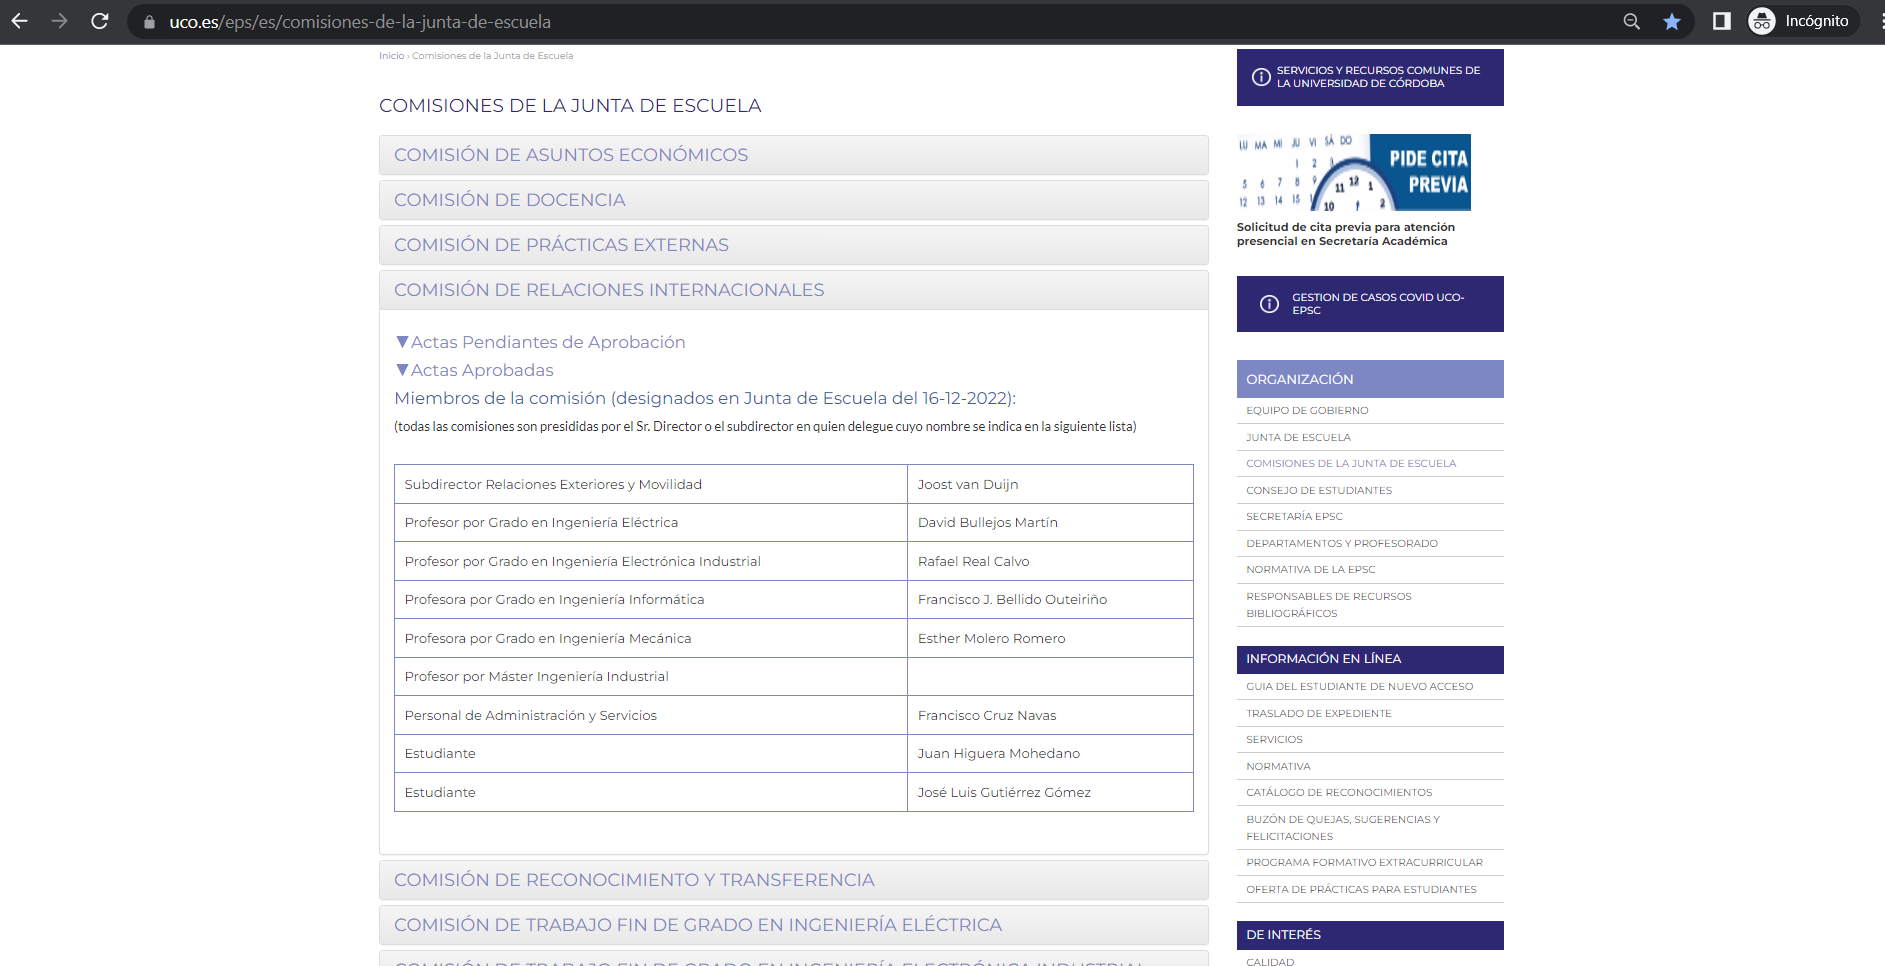
\includegraphics[scale=0.4]{img/capturas/WebComisionesEPSUCO.png}
    \caption{WEB: Información sobre los miembros de las comisiones de la EPS de la UCO}
    \label{fig:WebComisionesEPSUCO}
\end{figure}

\begin{figure}[H]
    \centering
    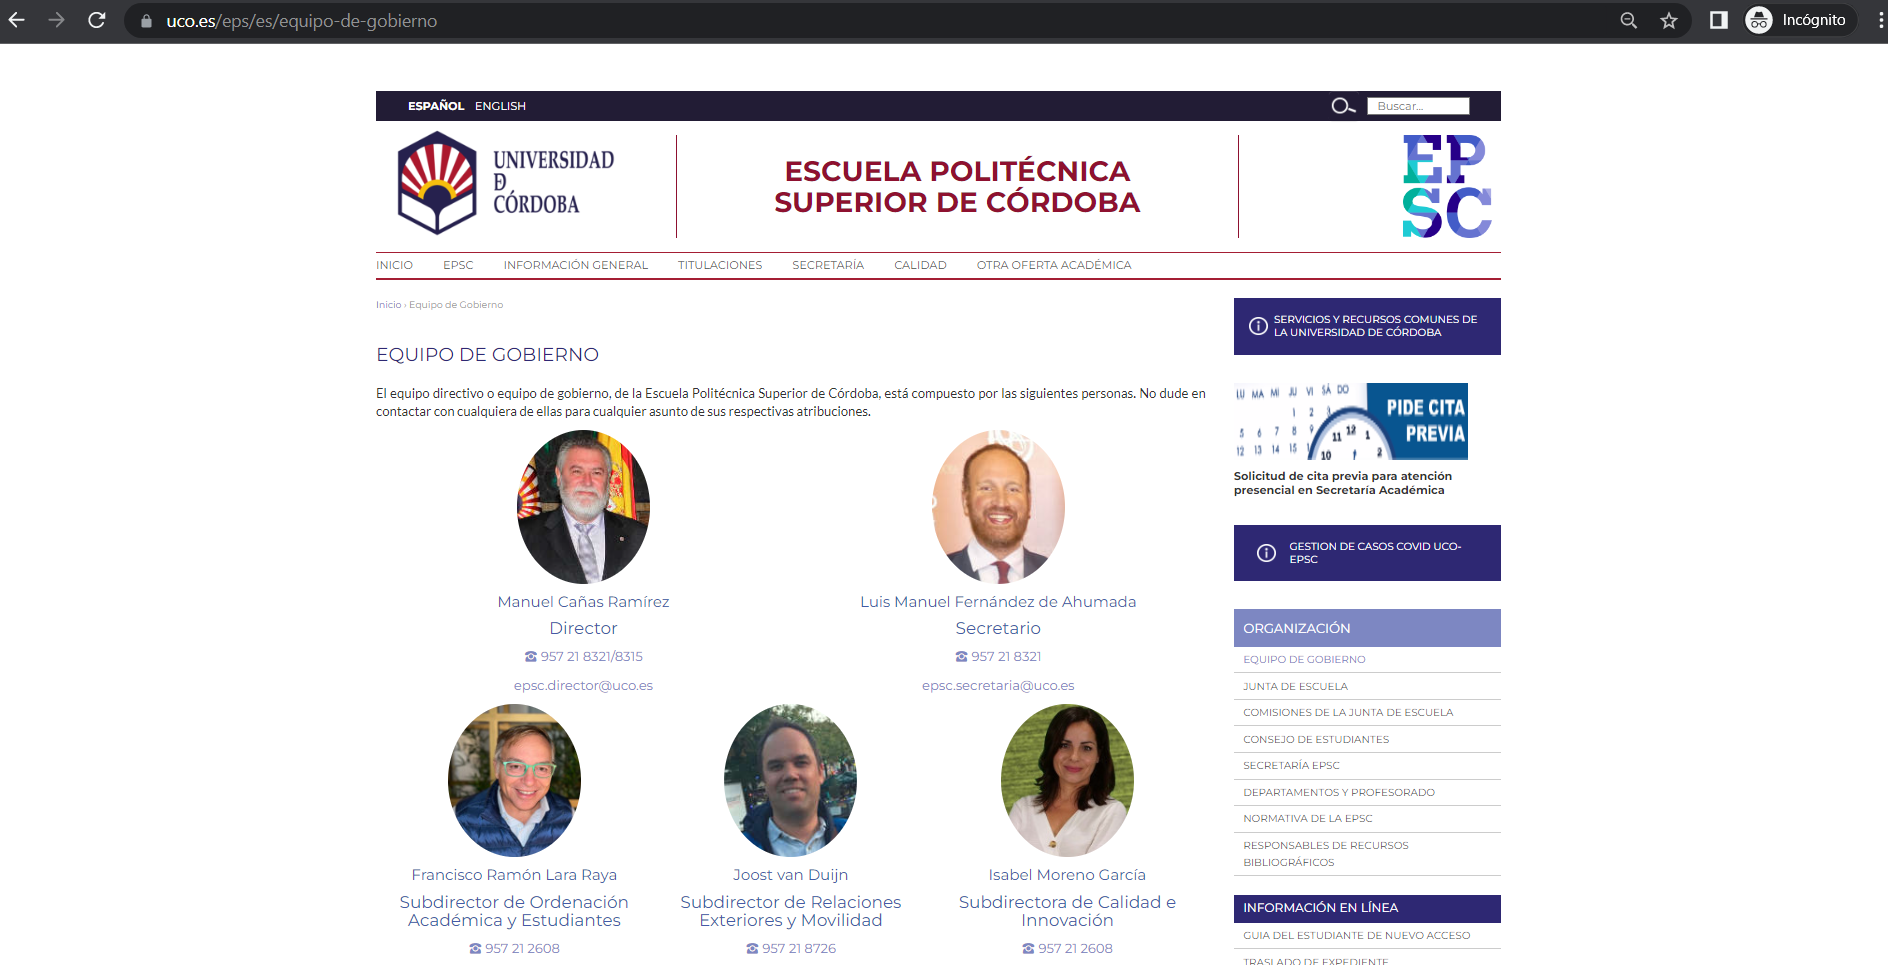
\includegraphics[scale=0.4]{img/capturas/WebEquipoGobiernoEPSUCO.png}
    \caption{WEB: equipo de gobierno de la EPS de la UCO}
    \label{fig:PACE-WebEquipoGobiernoEPSUCO}
\end{figure}

En definitiva, la Universidad de Córdoba carece de una aplicación web con una base de datos que permita asegurar la integridad de la información y evitar datos duplicados, ausentes o incorrectos. En la actualidad, se utilizan páginas web estáticas que deben ser mantenidas de forma individual, lo que provoca una gran carga de trabajo a los administrativos de los centros.

\section{Justificación del Trabajo de Fin de Grado}

El desarrollo del presente Trabajo de Fin de Grado está justificado porque no se tiene conocimiento de ninguna aplicación web que permita la gestión de comisiones de los distintos centros de la Universidad de Córdoba.

Actualmente, se realizan tareas manuales y estáticas sobre estas comisiones que provocan que la gestión administrativa sobre ellas sea una tarea lenta de realizar, sin conseguir una trazabilidad de cada uno de los cambios que pueden producirse a lo largo del tiempo y que repercute directamente en una pérdida de tiempo con respecto a utilizar un sistema que automatice lo máximo posible alguna de sus gestiones.
